\PassOptionsToPackage{unicode=true}{hyperref} % options for packages loaded elsewhere
\PassOptionsToPackage{hyphens}{url}
\PassOptionsToPackage{dvipsnames,svgnames*,x11names*}{xcolor}
%
\documentclass[]{article}
\usepackage{lmodern}
\usepackage{amssymb,amsmath}
\usepackage{ifxetex,ifluatex}
\usepackage{fixltx2e} % provides \textsubscript
\ifnum 0\ifxetex 1\fi\ifluatex 1\fi=0 % if pdftex
  \usepackage[T1]{fontenc}
  \usepackage[utf8]{inputenc}
  \usepackage{textcomp} % provides euro and other symbols
\else % if luatex or xelatex
  \usepackage{unicode-math}
  \defaultfontfeatures{Ligatures=TeX,Scale=MatchLowercase}
\fi
% use upquote if available, for straight quotes in verbatim environments
\IfFileExists{upquote.sty}{\usepackage{upquote}}{}
% use microtype if available
\IfFileExists{microtype.sty}{%
\usepackage[]{microtype}
\UseMicrotypeSet[protrusion]{basicmath} % disable protrusion for tt fonts
}{}
\IfFileExists{parskip.sty}{%
\usepackage{parskip}
}{% else
\setlength{\parindent}{0pt}
\setlength{\parskip}{6pt plus 2pt minus 1pt}
}
\usepackage{xcolor}
\usepackage{hyperref}
\hypersetup{
            pdftitle={LTE Cat-NB (Narrowband) Performance Evaluation},
            pdfauthor={Daniel Robinson},
            colorlinks=true,
            linkcolor=blue,
            citecolor=Blue,
            urlcolor=Blue,
            breaklinks=true}
\urlstyle{same}  % don't use monospace font for urls
\usepackage[left=3cm,right=3cm,top=2cm,bottom=2cm]{geometry}
\usepackage{longtable,booktabs}
% Fix footnotes in tables (requires footnote package)
\IfFileExists{footnote.sty}{\usepackage{footnote}\makesavenoteenv{longtable}}{}
\usepackage{graphicx,grffile}
\makeatletter
\def\maxwidth{\ifdim\Gin@nat@width>\linewidth\linewidth\else\Gin@nat@width\fi}
\def\maxheight{\ifdim\Gin@nat@height>\textheight\textheight\else\Gin@nat@height\fi}
\makeatother
% Scale images if necessary, so that they will not overflow the page
% margins by default, and it is still possible to overwrite the defaults
% using explicit options in \includegraphics[width, height, ...]{}
\setkeys{Gin}{width=\maxwidth,height=\maxheight,keepaspectratio}
\setlength{\emergencystretch}{3em}  % prevent overfull lines
\providecommand{\tightlist}{%
  \setlength{\itemsep}{0pt}\setlength{\parskip}{0pt}}
\setcounter{secnumdepth}{5}
% Redefines (sub)paragraphs to behave more like sections
\ifx\paragraph\undefined\else
\let\oldparagraph\paragraph
\renewcommand{\paragraph}[1]{\oldparagraph{#1}\mbox{}}
\fi
\ifx\subparagraph\undefined\else
\let\oldsubparagraph\subparagraph
\renewcommand{\subparagraph}[1]{\oldsubparagraph{#1}\mbox{}}
\fi

% set default figure placement to htbp
\makeatletter
\def\fps@figure{htbp}
\makeatother

\usepackage{float}
\usepackage{graphicx}
\usepackage{subfig}
\usepackage{chngcntr}

\counterwithin{figure}{section}

\let\origfigure\figure
\let\endorigfigure\endfigure
\renewenvironment{figure}[1][2] {
    \expandafter\origfigure\expandafter[H]
} {
    \endorigfigure
}

%% pandoc-tablenos: required package
\usepackage{caption}

%% pandoc-tablenos: environment to disable table caption prefixes
\makeatletter
\newcounter{tableno}
\newenvironment{tablenos:no-prefix-table-caption}{
    \caption@ifcompatibility{}{
    \let\oldthetable\thetable
    \let\oldtheHtable\theHtable
    \renewcommand{\thetable}{tableno:\thetableno}
    \renewcommand{\theHtable}{tableno:\thetableno}
    \stepcounter{tableno}
    \captionsetup{labelformat=empty}
    }
}{
    \caption@ifcompatibility{}{
    \captionsetup{labelformat=default}
    \let\thetable\oldthetable
    \let\theHtable\oldtheHtable
    \addtocounter{table}{-1}
    }
}
\makeatother

\title{LTE Cat-NB (Narrowband) Performance Evaluation}
\author{Daniel Robinson}
\date{Stellenbosch University, Sept 2019}

\begin{document}
\maketitle
\begin{abstract}
2G/GPRS is a sun-setting technology leaving behind a void for LPWANs
such as LoRaWAN and SigFox to fill. The viability of NB-IoT being such a
technology for South Africa is investigated. Multiple endpoint
manufacturers and base station vendors are tested to compare
capabilities with respect to power efficiency, latency, signal strength
and other metrics. The results proved promising.
\end{abstract}

{
\hypersetup{linkcolor=}
\setcounter{tocdepth}{3}
\tableofcontents
}
\listoftables
\listoffigures
\hypertarget{litstudy}{%
\section{Literature Study}\label{litstudy}}

Considering current literature, several studies provide theoretical
models not only for the energy consumption of NB-IoT networks
{[}\protect\hyperlink{ref-Andres-Maldonado2017}{1}{]}, but also for
their latency and delay bounds
{[}\protect\hyperlink{ref-Feltrin2019}{2}{]}, impact of coverage
extensions {[}\protect\hyperlink{ref-Andres-Maldonado2018b}{3}{]},
coverage performance {[}\protect\hyperlink{ref-Adhikary2016}{4}{]},
battery lifetimes
{[}\protect\hyperlink{ref-Yeoh2018d}{5}{]},{[}\protect\hyperlink{ref-Lauridsen2018}{6}{]},
theoretically optimal configuration strategies
{[}\protect\hyperlink{ref-Feltrin2018}{7}{]} and overall performance for
particular verticals
{[}\protect\hyperlink{ref-Soussi2018}{8}{]},{[}\protect\hyperlink{ref-Beyene2017b}{9}{]}.

Only Martinez {[}\protect\hyperlink{ref-Martinez2019}{10}{]} focuses
effort on the adopter and presents an operational and empirical analysis
of the technology when it is deployed in a real network (such as
Vodafone in the Metropolitan area of Barcelona). Durand
{[}\protect\hyperlink{ref-Thomas2018}{11}{]} compares different LPWANs
empirically including NB-IoT. Despite the unquestionable value of the
theoretical models (for example, to understand orders of magnitude or to
guess the theoretical upper and lower bounds), an empirical approach
provides real insights into the variability that a UE device experiences
when deployed in real conditions. This work therefore complements
Martinez and related works, and it further provides empirical
measurements for UEs that are deployed using a real-world NB-IoT network
always while taking the perspective of an application developer.

\begin{itemize}
\tightlist
\item
  GSM RF equipment testing and performance analysis
  {[}\protect\hyperlink{ref-Kasbah2005}{12}{]}
\item
  Analysis of NB-IoT Deployment in LTE Guard-Band
  {[}\protect\hyperlink{ref-Ratasuk2017c}{13}{]}
\end{itemize}

Whilst this research is funded by MTN and being aware of internal
documentation, this is an independent study which should aid any
potential adopters of the technology.

The empirical results of NB-IoT depend on the device used (UE) and
underlying LTE vendor architecture of the MNO providing coverage. Thus,

\hypertarget{lorawan}{%
\subsection{LoRaWAN}\label{lorawan}}

LoRaWAN is a contender for NB-IoT. It lacks bidirectionality and data
rate.

\begin{itemize}
\tightlist
\item
  LoRaWAN performs better for short messages, but it is subjected to a
  very high penalty when more than one message per data block is
  required.
\item
  Second, the LoRaWAN reliability mechanism must be ensured at the upper
  layers, and thus may incur higher energy costs.
\end{itemize}

\hypertarget{dash7}{%
\subsection{Dash7}\label{dash7}}

\hypertarget{sigfox}{%
\subsection{SigFox}\label{sigfox}}

SigFox is a contender for NB-IoT. It lacks bidirectionality and
datarate.

\hypertarget{nbiot_lit}{%
\subsection{NB-IoT}\label{nbiot_lit}}

\begin{itemize}
\tightlist
\item
  This section describes NB-IoT in more detail and the setup procedures
  involved.
\item
  3GPP
\item
  the UE device is to a large extent/entirely controlled by the
  network/eNodeB.

  \begin{itemize}
  \tightlist
  \item
    UE devices must follow NW settings broadcast inside the SIB and
    allocations for UL/DL data.
  \end{itemize}
\end{itemize}

Martinez {[}\protect\hyperlink{ref-Martinez2019}{10}{]} has explored
NB-IoT from the perspective of the application developer. When
evaluating performance, it would do well to find the limits of the
technology as well as find the optimum `sweet spot' or range for
efficient operation.

A user would consider critical characteristics such as energy
consumption, coverage, cost, network latency and behavior. Martinez
looks at these except for cost, which is better looked at by Ali
{[}\protect\hyperlink{ref-Ali2015}{14}{]}. A set of tests were devised
and results showed that in some cases its energy consumption performed
better than an LPWAN referenced technology such as LoRa, with the added
benefit of guaranteeing delivery. However, the high variability in
energy consumption and network latency call into question its
reliability especially for mission-critical applications.

\hypertarget{lit_standing}{%
\subsection{Standing or Positioning}\label{lit_standing}}

We expect selected uptake of each technology in specific application
areas and our results show that each technology is better suited to
specific applications and their concomitant requirements. Sigfox,
NB-IoT, and LoraWAN SF12 performed equally well for applications where
MCL (range) is paramount, with LoraWAN SF7 doing slightly worse. In
applcitions where the main consideration is scalability, Sigfox, and
NB-IoT substantially outperformed the LoraWAN varieties. However, if
battery life is the most important consideration, LoraWAN SF7 seems to
have the edge, with NB-IoT (the default setup we tested) performing
worse. NB-IoT performed the best for uplink throughput, with LoraWAN SF7
coming in second. For all the other two-related metrics evaluated,
namely downlink throughput and firmware upgradability, NB-IoT performs
substantially better than the other technologies.

\begin{itemize}
\tightlist
\item
  Comparison
\end{itemize}

{[}\protect\hyperlink{ref-Martinez2019}{10}{]}

NB-IoT has proven to be competitive in terms of energy consumption,

\begin{itemize}
\tightlist
\item
  Decent study on the operational trade-offs of NB-IoT over LTE.
\end{itemize}

Complexities

\begin{itemize}
\tightlist
\item
  signalling, dynamic adjustments triggered by network conditions,
  timing
\item
  competitive in terms of NB-IoT consumption due to 3GPP efforts to be
  similar to LPWANs
\end{itemize}

Proprietary spectrum vs ISM bands?

\begin{itemize}
\tightlist
\item
  ISM external interference and share
\item
  otherwise high unpredictability in device behavior
\end{itemize}

Reliability?

\begin{itemize}
\tightlist
\item
  Delivery guarantee
\end{itemize}

Delay Tolerance

\begin{itemize}
\tightlist
\item
  high variability in delivery time. Deal-breaker for some applications.
\end{itemize}

Data rate

\begin{itemize}
\tightlist
\item
  sporadic high bandwidth
\end{itemize}

Ownership model

\begin{itemize}
\tightlist
\item
  connectivity service, contract, charged per byte
\item
  coverage depends on deployed infrastructure
\end{itemize}

\hypertarget{lit_hardware}{%
\subsection{Hardware}\label{lit_hardware}}

\begin{itemize}
\tightlist
\item
  Modem
\item
  Antenna
\item
  RX/TX lines
\end{itemize}

\hypertarget{lit_setup}{%
\subsection{Setup Procedure}\label{lit_setup}}

\begin{itemize}
\tightlist
\item
  There exist application development manuals.
\item
  AT+NCONFIG

  \begin{itemize}
  \tightlist
  \item
    AUTOCONNECT
  \item
    CR\_0859\_SI\_AVOID
  \item
    CR\_0354\_0338\_SCRAMBLING
  \end{itemize}
\item
  URCs
\item
  APN
\end{itemize}

\hypertarget{nw_reg_info}{%
\subsection{Network Registration and Info}\label{nw_reg_info}}

\begin{itemize}
\item
  By default the SARA-N2 series modules will automatically try and
  connect to the network. This feature will read the SIM for the PLMN
  and attempt to register with the network. The device will use the
  default APN from the network. The auto-connect feature can be enabled
  by the +NCONFIG AT command. Reset the module to save these settings to
  the non-volatile memory.
\item
  If the application requires more control over the registration process
  set the SARA-N2 series modules into the manual registration mode. With
  the auto-connect feature turned off the module is able to manually
  connect to a specific PLMN and specify an APN.
\item
  After a RRC connection is made to the base station the module will try
  and register with the network. If the module IMEI or IMSI is not
  allowed on the network, the module will disconnect from that base
  station and continue scanning for other base stations. This can be
  seen if the parameter of the +CSCON AT command shows the ``1'' and
  then ``0'' response without +CEREG changing to 1 or 5 means that the
  module was not able to register on that network. In case the module is
  registered to the network, the parameter of the +CEREG AT command will
  be 1 (registered) or 5 (registered \& roaming).
\item
  See {[}\protect\hyperlink{ref-ubloxAppNote2018}{15}{]}{]} for a
  connection status compatibility matrix.
\item
  PCI value is assigned.
\end{itemize}

The \textbf{PCI} value is created from two components - PSS and SSS. The
PSS, Primary Synchronization Signal, has the value 0, 1, or 2. The SSS,
Secondary Synchronization Signal, can have a value between 0 and 167.

\hypertarget{rrc_inactivity}{%
\subsection{RRC Connection and Inactivity Timer}\label{rrc_inactivity}}

After network registration or transmitting a data packet, the device
usually enters RRC connected (C-DRX) mode for a specified inactivity
timeout specified by the network.

\begin{itemize}
\tightlist
\item
  When the module is in RRC connected mode it will be receiving all the
  base station signaling. The average power consumed in this mode is
  about 48 mA. If the RRC connection is left for 20 s of inactivity
  before the RRC is released, then this will consume about 1 mWh @ 3.6V.
\item
  48 mA in this mode
\item
  20 seconds is about 1mWh @ 3.6V
\item
  AT+CSCON
\item
  After a short period, if no messages are being sent from the module,
  the +CSCON response will be ``0'' to show the RRC connection has been
  released by the eNodeB.
\item
  At the first registration or when the module wakes from the power save
  mode (PSM), it performs a Random Access CHannel (RACH) procedure to
  attach to the base station. This establishes a Radio Resource Control
  (RRC) connection to the base station. Once established only the base
  station can release this connection. The module cannot drop the RRC
  connection other than turning off the radio using the AT+CFUN=0
  command.
\item
  The base station has an ``inactivity'' timer for each module and if
  there is no activity the base station will send a RRC release message
  to the module. The module should respond back to the base station with
  an acknowledgment. The inactivity timer is nominally 20 s.
\item
  The module will be able to receive and send messages immediately when
  in connected mode.
\item
  During a RRC connection, the +CSCON AT command provide the signalling
  connection status. It is also possible to enable the +CSCON URC.
\item
  When a MO message is sent from the module, the module must first
  create a RRC connection if there is not already established with the
  base station. This status can be checked using the AT+CSCON command.
  To check the signalling connection status issue the +CSCON read
  command. The second parameter of the information text response
  (+CSCON: ,) provides the interested information:

  \begin{itemize}
  \tightlist
  \item
    0: idle mode (no RRC connection)
  \item
    1: connected mode (RRC connection)
  \end{itemize}
\item
  To configure a URC for this command, issue the AT+CSCON=1 command. A
  URC will be issued at each RRC connection status change.
\end{itemize}

\hypertarget{release_a}{%
\subsection{Release Assistance}\label{release_a}}

Release assistance requests the eNodeB to release the RRC connection
immediately. By avoiding 20 seconds of idle RRC in C-DRX mode, there is
a 93\% improvement in power consumption for a 200 byte transmission in
ECL 1.

{[}\protect\hyperlink{ref-ubloxAppNote2018}{15}{]}

An example of sending a 200 byte message in ECL 2 with good SNR can
include 5 RACH transmission bursts, a Transmission Block Size
\textasciitilde{}43 bytes, one repetition and taking just over 1 second,
consuming 200uWh.

For the same example in bad SNR, the TBS allocated 32 bytes per chunk,
with a repetition of 8 and 4. It took 5.5 seconds and consumed 1.07mWh
-- fives times as much as before.

\begin{itemize}
\tightlist
\item
  Some applications may not want to wait for the base station's
  inactivity timer to expire after 20 s as this wastes power from the
  battery. In Release-13 the ``Release Assistance'' feature allows the
  module to request for the RRC connection to be dropped as soon as the
  message has been received by the network.
\item
  The flag is noticed by the MME on the network and sends a message back
  to the eNodeB base station to drop the RRC connection. The network
  must support Release Assistance for this feature.
\item
  After the RRC connection has been released the module then goes in to
  a period where it could be paging the base station. The timer for this
  period is called T3324. After T3324 has expired the module goes into
  Power Save Mode (PSM). See section 11 for further information
\end{itemize}

\hypertarget{power-saving-mechanisms}{%
\subsection{Power Saving Mechanisms}\label{power-saving-mechanisms}}

The NB-IoT protocol allows for power save mode (PSM), and the SARA-N2
series modules also support a Deep Sleep mode where the module is
running at very low current, \textasciitilde{}3 \(uA\). The module
automatically enters various states depending on the device activity.
Here below are listed the common activities and the various states it
will be in after registration.

\begin{itemize}
\tightlist
\item
  T3324 / T3412 timer values
\end{itemize}

\hypertarget{t3412-ptau-timer}{%
\subsubsection{T3412 PTAU Timer}\label{t3412-ptau-timer}}

\begin{itemize}
\item
  (GPRS timer 3)
\item
  3GPP TS 24.008 {[}4{]}, figure 10.5.147a and table 10.5.163a.
\item
  Bits 5 to 1 represent the binary coded timer value. Bits 6 to 8 define
  the timer value unit for the GPRS timer as follows
\item
  8 7 6 0 0 0 value is incremented in multiples of 10 minutes 0 0 1
  value is incremented in multiples of 1 hour 0 1 0 value is incremented
  in multiples of 10 hours 0 1 1 value is incremented in multiples of 2
  seconds 1 0 0 value is incremented in multiples of 30 seconds 1 0 1
  value is incremented in multiples of 1 minute 1 1 0 value is
  incremented in multiples of 320 hours (Note 1) 1 1 1 value indicates
  that the timer is deactivated (Note 2)
\item
  Example: ``01000111'' = 7 x10 hours = 70 hours
\item
  NOTE 1: This timer value unit is only applicable to the T3312 extended
  value IE and the T3412 extended value IE (see 3GPP TS 24.301 {[}5{]}).
  If it is received in an integrity protected message, the value shall
  be interpreted as multiples of 320 hours. Otherwise the value shall be
  interpreted as multiples of 1 hour.
\item
  NOTE 2: This timer value unit is not applicable to the T3412 extended
  value IE. If this timer value is received, the T3412 extended value IE
  shall be considered as not included in the message (see 3GPP TS 24.301
  {[}5{]}).
\end{itemize}

\hypertarget{t3324-active-timer}{%
\subsubsection{T3324 Active Timer}\label{t3324-active-timer}}

\begin{itemize}
\item
  The T3324 Timer is reset after a downlink message is received. The
  negative impact on energy savings should be taken into account if
  downlink data is fragmented.
\item
  the Active Timer (T3324) controls the time lapse during which the UE
  device is reachable by the network in RRC Idle, i.e., the number of
  eDRX cycles.
\item
  Bits 5 to 1 represent the binary coded timer value. Bits 6 to 8 define
  the timer value unit for the GPRS timer as follows
\item
  8 7 6 0 0 0 value is incremented in multiples of 2 seconds 0 0 1 value
  is incremented in multiples of 1 minute 0 1 0 value is incremented in
  multiples of deci-hours 1 1 1 value indicates that the timer is
  deactivated
\item
  Example: ``00100100'' = 4 x1 minute = 4 minutes
\end{itemize}

\hypertarget{edrx-cycles-and-ptw}{%
\subsubsection{eDRX Cycles and PTW}\label{edrx-cycles-and-ptw}}

\begin{itemize}
\tightlist
\item
  An eDRX cycle is composed of an active phase, controlled by a Paging
  Time Window (PTW) timer, which ranges from 2.56 s to 40.96 s followed
  by a sleep phase until the end of the eDRX cycle. Within the PTW, the
  standard LTE paging is observed.
\end{itemize}

Extended Discontinuous Reception (eDRX) mode means that paging windows
can be scheduled such that the modem can be contacted by the server.

\begin{figure}
\centering
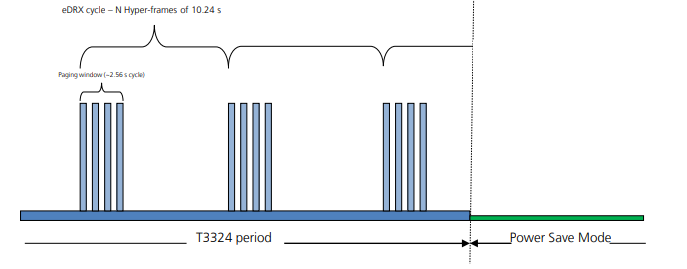
\includegraphics{C:/Users/d7rob/AppData/Roaming/Typora/typora-user-images/1555540836196.png}
\caption{eDRX mode}
\end{figure}

\hypertarget{sib}{%
\subsection{System Information Blocks (SIB)}\label{sib}}

The SIB describes the method of attachment and what repetitions the UE
device must use to first transmit to the base station. Once a RRC
connection is made, the base station then uses the perceived SNR to
configure the uplink allocations the UE device will use to transmit the
messages. Because allocations for each uplink/downlink are dynamically
set by the base station it is difficult to calculate the power
consumption of a single message deployed in the field.

\begin{itemize}
\tightlist
\item
  example SIB
\end{itemize}

\hypertarget{repetitions-and-extended-coverage-level-ecl}{%
\subsection{Repetitions and Extended Coverage Level
(ECL)}\label{repetitions-and-extended-coverage-level-ecl}}

\begin{itemize}
\item
  ECL
\item
  Module interference increases the number of repetitions
\item
  Minimize ECL 2.
\item
  Network operators should provide enough coverage to allow devices to
  be mostly in coverage class 0 or 1. Depending on the NB-IoT
  deployment, the network could have large areas, or devices located in
  deep locations which unfortunately mean they operate in Coverage Class
  2.
\item
  Coverage Class 2 uses high repetitions for the RACH process and also
  higher coding schemes when transmitting data and therefore
  fundamentally consumes more power than it would in the other coverage
  classes.
\item
\end{itemize}

\hypertarget{ue-device-and-network-behavior}{%
\subsection{UE Device and Network
Behavior}\label{ue-device-and-network-behavior}}

\begin{itemize}
\tightlist
\item
  The application can monitor the status of the module's connection,
  registration and PSM state by polling or configuring URCs. By
  monitoring the module status the application can behave more
  efficiently, depending on the application type. For example, the
  application may want to know when the module goes into Power Save Mode
  (PSM).
\end{itemize}

Register the module to the NB-IoT network before to send or receive any
messages. Without being registered the module will not be able to send
or receive any messages. To check the network registration status issue
the +CEREG read command. The second parameter of the information text
response (+CEREG: ,) provides the interested information * 0: not
registered, not registering * 1: registered * 2: not registered, but
currently in the process to * 3: registration denied. The application
should have a re-try mechanism which does not simply try registration
immediately, but has some back-off process * 4: unknown * 5: registered,
roaming

When the module has started the network search process, poll the
+NUESTATS AT command and view the Rx and Tx Time:

\begin{itemize}
\tightlist
\item
  If Rx Time is increasing then the module is trying to scan for a base
  station.
\item
  If Tx Time is increasing then the module has found a base station and
  is trying to communicate with it.
\item
  If the Total Power and Signal Power values are different than -32767
  (invalid) then the module has read the MIB and SIB signals from the
  base station.
\item
  Once an RRC connection is made, the +CSCON read command will return 1.
  Turn on the +CSCON URC which will be output at each RRC connection
  change.
\end{itemize}

If the SIM used is an international SIM (roaming SIM) then the
registration process can take many minutes for the first time. Once the
module is registered on that network the PLMN should be stored in the
SIM so that registration is quicker next time. The application can tell
if it is using roaming SIM by the state being ``5''.

\begin{itemize}
\tightlist
\item
  The +CEREG URC can be enabled to provide the network registration
  status. Depending on the parameter it is possible to configure the
  interested URC parameters (i.e. =4 or 5 to see the provided network
  timers). See SARA-N2 AT Commands Manual {[}2{]} for more details.
\item
  Properly setting the +CEREG AT command (=3, 4 or 5) it is possible to
  see the registration EMM cause value. These values are described in
  the 3GPP TS 24.008 {[}4{]}. Typical causes:

  \begin{itemize}
  \tightlist
  \item
    \#5 IMEI not accepted
  \item
    \#11 PLMN not allowed
  \item
    \#12 Location Area not allowed
  \item
    \#13 Roaming not allowed in this location area
  \item
    \#22 Congestion
  \end{itemize}
\end{itemize}

\hypertarget{data-transmission}{%
\subsection{Data transmission}\label{data-transmission}}

The SARA-N2 series modules are able to send raw data through UDP sockets
to an IP address. The data sent over the socket AT commands is not
wrapped in any other layer, and the data provided is the data that is
sent.

The Constrained Application Protocol (CoAP) is a datagram-based
client/server application protocol for devices on the constrained
network (e.g.~low overhead, low-power), designed to easily translate to
HTTP for simplified integration with the web. CoAP clients can use the
GET, PUT, POST and DELETE methods using requests and responses with a
CoAP server.

The usage of the Non-IP method during the sending or receiving of
messages saves the overhead of needing to send a UDP IP header.

See {[}\protect\hyperlink{ref-ubloxAppNote2018}{15}{]} for an
Application example.

\hypertarget{ping}{%
\subsubsection{Ping}\label{ping}}

Issue the +NPING AT command to check if the module is able to send and
receive data. Check to see if the network can communicate to the
internet, or it is needed another accessible server's IP address to
ping. To ping Google's DNS server: AT+NPING=``8.8.8.8'' To ping OpenDNS
DNS server: AT+NPING=``208.67.222.222'' The information text response to
the +NPING AT command will be issued after a few seconds. If the
information text response is +NPINGERR: 1, the ping has timed out.

\begin{itemize}
\tightlist
\item
  The first ping might fail because it can take a few seconds to connect
  to the base station. Use the +CSCON URC to show when the module is
  connected.
\end{itemize}

\hypertarget{echo}{%
\subsubsection{Echo}\label{echo}}

For a more advanced check on sending data to an external server, send
data to the u-blox echo server at echo.u-blox.com. * Because there is no
DNS lookup function in the SARA-N2 module series, use the IP address
server which is 195.34.89.241.

Command Response Description AT+NSOCR=``DGRAM'',17,10000 0 OK Create a
UDP socket. AT+NSOST=0,``195.34.89.241'',7,5,``0102 030405'' 0,5 OK Send
data on socket 0. +NSONMI: 0,5 Receive data on socket 0. AT+NSORF=0,5
+NSORF: 0,``195.34.89.241'',7,5 ,``0102030405'',0 OK Request data from
socket 0. Echo'd data received

\hypertarget{available-metrics}{%
\subsection{Available Metrics}\label{available-metrics}}

When the module is synchronized to the base station and is receiving the
signaling the +NUESTATS AT command is able to describe the radio, cell,
BLER and throughput statistics. The most useful statistic is the
``RADIO'' type.

\hypertarget{rsrp}{%
\subsubsection{RSRP}\label{rsrp}}

It is the power of the wanted part of the receive signal, the NB-IoT
part.

\hypertarget{total-power}{%
\subsubsection{Total power}\label{total-power}}

It is the radio signal strength within the receive bandwidth (both
expressed in 10ths of a decibel). From this the signal to noise ratio
can be calculated.

\hypertarget{transmit-power}{%
\subsubsection{Transmit power}\label{transmit-power}}

\begin{itemize}
\item
  It is the RF power output from the module. It may be a low number if
  the received signal strength is good (and hence the module assumes
  that the base station is close by).
\item
  Ideally the module should consume 230 mA for +23 dBm.
\end{itemize}

\hypertarget{tx-rx-time}{%
\subsubsection{TX, RX Time}\label{tx-rx-time}}

TX Time is the duration for which the module's transmitter has been
switched on.

RX Time is the duration for which the module's receiver has been
monitored for downlink activity (both expressed in milliseconds since
the last reboot). Together these can be used to assess the time the
module spends in each state and hence estimate the power consumed by the
module.

When the module first tries to register with the network, the Tx time
will be zero as it will not have instantly found a base station. The Rx
time will increase to show it is scanning for a base station. Once a
base station is found it is possible to see that it is attempting to
transmit to the base station as the Tx time will start to increase. If
the base station does not respond to the module's Tx, then the +CSCON: 1
URC will not be issued.

\hypertarget{ecl}{%
\subsubsection{ECL}\label{ecl}}

It is equivalent to ``PRACH coverage enhancement level'' defined in 3GPP
36.321 {[}3{]} sub clause 5.1

\begin{itemize}
\tightlist
\item
  As observed, the ECL has an impact on energy consumption, but not on
  the delay.
\end{itemize}

\hypertarget{snr}{%
\subsubsection{SNR}\label{snr}}

Last SNR value.

\hypertarget{latency}{%
\subsection{Latency}\label{latency}}

\begin{itemize}
\item
  \textless{} 10 seconds
\item
\end{itemize}

\hypertarget{power}{%
\subsection{Power Consumption}\label{power}}

\begin{itemize}
\tightlist
\item
  \textasciitilde{} 10 years battery life
\end{itemize}

Low power consumption is vital for battery longevity.

\begin{itemize}
\tightlist
\item
  PCB layout, antenna matching and location will have an effect to the
  overall interference received by the module.
\item
  PSM and eDRX
\item
  On the other hand, although the average power is comparable, peaks in
  transmission of LoRaWAN's radio are around 40 mA, while in NB-IoT they
  reach 220 mA. This causes additional stress on the battery, which has
  to be managed with care.
\item
  As can be observed, mean values for NB-IoT are similar to the energy
  that a LoRaWAN device requires to transmit while using the SF12
  configuration. The 5th percentile results for NB-IoT (best observed
  performance) are comparable to the best case performance of LoRaWAN
  when operating at SF8. This is in our opinion a relevant result, as
  NB-IoT guarantees packet delivery with similar power consumption.
\item
  The expected achievable lifespan (on average) for a NB-IoT is on the
  order 2-3 years, depending on the datagram size.
\item
  However, adopters may take into consideration some differences. First,
  sending larger messages (up to 512 bytes) has almost no impact on
  NB-IoT.
\item
  In a simple periodic-reporting application with very limited computing
  requirements5, the average power can be modeled approximately by Eq.
  \ref{eq:avgpower}, as detailed in {[}21{]}:
\end{itemize}

\begin{equation}P = \frac{E_{msg}}{T_{msg}}\label{eq:avgpower}\end{equation}

\begin{itemize}
\item
\end{itemize}

\hypertarget{data-usage}{%
\subsection{Data Usage}\label{data-usage}}

\begin{itemize}
\tightlist
\item
  The module has a limited dynamic message queue size. For IoT
  applications, the message size should be of the order of tens of
  bytes. UDP socket commands limit their payload size to 512 bytes.
\item
  There is no indication when the UDP data has been sent.
\item
  Downlink data from the cloud server must also be 512 bytes or less,
  because otherwise the messages will be lost.
\item
  The module has an internal message buffer. If the module is unable to
  send the messages to the network before this buffer is full, because
  the application is queueing quicker than it can send them, then the UE
  device will return ERROR for the +NSOST/+NSOSTF commands.
\item
  If a message cannot be sent because of communication issues between
  the module and eNB, the module will attempt to send the message a
  second time. If this fails, the message will be dropped. As
  +NSOST/+NSOSTF messages are UDP, there is no indication the message
  has been dropped.
\item
  The UDP header is about 48-60 bytes in length, and so an application
  sending 100 bytes will actually send about 160 bytes. For devices in
  the extreme coverage class 2, this can be quite costly.
\item
  The UE device may later resume the RRC Connected state with that
  context, thus avoiding the AS setup and saving considerable signaling
  overhead for the transmission of infrequent small data packets.
\end{itemize}

\hypertarget{application-architecture}{%
\subsection{Application Architecture}\label{application-architecture}}

\begin{itemize}
\tightlist
\item
  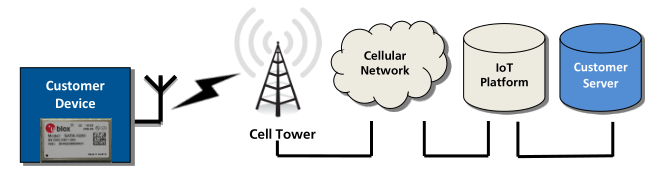
\includegraphics{../images/1569744612309.png}
\item
  At the far left the customer's device contains a u-blox NB-IoT module
  that communicates over the radio network with a cell tower that
  supports the NB-IoT network. The cellular network links the cell tower
  with an IoT platform. This IoT platform stores uplink datagrams from
  the NB-IoT module. The customer server communicates with the IoT
  platform to retrieve uplink datagrams and to send downlink datagrams
  to the NB-IoT. The IoT platform holds downlink datagrams until the
  NB-IoT module is awake to receive them.
\item
  The SARA-N2 series modules implement basic UDP socket commands for
  directly communicating with an external service. With these commands
  the customer can build a simple IoT platform. With an external
  processor other IoT layers could be implemented to aid this system
  design. SARA-N2 series modules support AT commands for general CoAP
  messaging. This allows the customer to not require CoAP in their
  external processor.
\item
  Many developers coming from a GPRS type background may expect an
  always on type connection, normally using TCP. NB-IoT is not session
  oriented, latencies are much higher and the device will enter a power
  save mode. This is very different to always-on modems with ``chatty''
  protocols like TCP.
\item
  UDP sockets do not create connections to servers; UDP is a
  connection-less datagram protocol. Because of this MO messages may not
  be received by the server and lost. The application should take this
  in to consideration and provide its own acknowledgements between the
  UE device and server. CoAP is one protocol which can be used on top of
  UDP to provide this.
\item
  For resolving the issue of sending MT messages to a very sleepy
  module, when a MO message is sent to the cloud server, the cloud
  server will know the module is active and connected to the network. As
  seen in section 7 the connection is alive until the RRC connection is
  released by the network and then still contactable when paging inside
  the T3324 period. If there are MT messages to be sent to the module,
  the cloud server should send this message in this time.
\end{itemize}

\hypertarget{use-cases}{%
\subsection{Use cases}\label{use-cases}}

Use cases suitable for NB-IoT

\hypertarget{martinez}{%
\subsection{Martinez}\label{martinez}}

Martinez et al. {[}\protect\hyperlink{ref-Martinez2019}{10}{]} did
empirical tests within the Vodafone Network in Barcelona. They observed
UE device and NW behavior, measured current traces, and did various
tests in different modes.

\begin{longtable}[]{@{}ll@{}}
\caption{NW Config \label{tbl:nw_config}}\tabularnewline
\toprule
\begin{minipage}[b]{0.13\columnwidth}\raggedright
Mode\strut
\end{minipage} & \begin{minipage}[b]{0.81\columnwidth}\raggedright
NW Configuration\strut
\end{minipage}\tabularnewline
\midrule
\endfirsthead
\toprule
\begin{minipage}[b]{0.13\columnwidth}\raggedright
Mode\strut
\end{minipage} & \begin{minipage}[b]{0.81\columnwidth}\raggedright
NW Configuration\strut
\end{minipage}\tabularnewline
\midrule
\endhead
\begin{minipage}[t]{0.13\columnwidth}\raggedright
\textbf{Mode 1}\strut
\end{minipage} & \begin{minipage}[t]{0.81\columnwidth}\raggedright
Inactivity timer = 20s (network default)T3324 = 0s (disabled)C-DRX =
2.048s (network default)\strut
\end{minipage}\tabularnewline
\begin{minipage}[t]{0.13\columnwidth}\raggedright
\textbf{Mode 2}\strut
\end{minipage} & \begin{minipage}[t]{0.81\columnwidth}\raggedright
Inactivity timer = Immediate ReleaseT3324 = 8sI-DRX = 2.56seDRX/PTW =
Disabled\strut
\end{minipage}\tabularnewline
\begin{minipage}[t]{0.13\columnwidth}\raggedright
\textbf{Mode 3}\strut
\end{minipage} & \begin{minipage}[t]{0.81\columnwidth}\raggedright
Inactivity timer = Immediate ReleaseT3324 = 0s (disabled)\strut
\end{minipage}\tabularnewline
\bottomrule
\end{longtable}

\begin{itemize}
\tightlist
\item
  performance bounds
\item
  empirical
\end{itemize}

\hypertarget{notes}{%
\subsection{Notes}\label{notes}}

\textbf{MTN Lab / 14th Ave Phase 3: Test Plant}

NB-IoT PoC MTN South Africa (Ericsson RAN Connectivity Tests only)
{[}\protect\hyperlink{ref-Ssengonzi2017}{16}{]}

Industrial north Drive Test Requirements
{[}\protect\hyperlink{ref-NorthDrive2017}{17}{]}

\textbf{Stellenbosch}

Evaluation of next-generation low-power communication technologies to
replace GSM in IoT-applications
{[}\protect\hyperlink{ref-Thomas2018}{11}{]}

\textbf{Manufacturers}

Ublox has an NB-IoT Application Development Guide
{[}\protect\hyperlink{ref-ubloxAppNote2018}{15}{]} which details many of
the capabilities of the UE.

\hypertarget{refs}{}
\leavevmode\hypertarget{ref-Andres-Maldonado2017}{}%
{[}1{]} P. Andres-Maldonado, P. Ameigeiras, J. Prados-Garzon, J.
Navarro-Ortiz, and J. M. Lopez-Soler, ``Narrowband IoT Data Transmission
Procedures for Massive Machine-Type Communications,'' \emph{IEEE
Network}, vol. 31, no. 6, pp. 8--15, 2017.

\leavevmode\hypertarget{ref-Feltrin2019}{}%
{[}2{]} L. Feltrin, G. Tsoukaneri, M. Condoluci, C. Buratti, T.
Mahmoodi, M. Dohler, and R. Verdone, ``Narrowband IoT: A survey on
downlink and uplink perspectives,'' \emph{IEEE Wireless Communications},
vol. 26, no. 1, pp. 78--86, 2019.

\leavevmode\hypertarget{ref-Andres-Maldonado2018b}{}%
{[}3{]} P. Andres-Maldonado, P. Ameigeiras, J. Prados-Garzon, J. J.
Ramos-Munoz, J. Navarro-Ortiz, and J. M. Lopez-Soler, ``Analytic
analysis of narrowband IoT coverage enhancement approaches,'' \emph{2018
Global Internet of Things Summit, GIoTS 2018}, 2018.

\leavevmode\hypertarget{ref-Adhikary2016}{}%
{[}4{]} A. Adhikary, X. Lin, Y. P. Eric Wang, Y. .. E. Wang, and Y. P.
Eric Wang, ``Performance evaluation of NB-IoT coverage,'' in \emph{IEEE
vehicular technology conference}, 2017, pp. 1--5.

\leavevmode\hypertarget{ref-Yeoh2018d}{}%
{[}5{]} C. Y. Yeoh, A. bin Man, Q. M. Ashraf, A. K. Samingan, A. Bin
Man, Q. M. Ashraf, A. K. Samingan, A. bin Man, Q. M. Ashraf, A. K.
Samingan, A. Bin Man, Q. M. Ashraf, and A. K. Samingan, ``Experimental
assessment of battery lifetime for commercial off-the-shelf NB-IoT
module,'' in \emph{2018 20th international conference on advanced
communication technology (icact)}, 2018, vols. 2018-Febru, p. 1.

\leavevmode\hypertarget{ref-Lauridsen2018}{}%
{[}6{]} M. Lauridsen, R. Krigslund, M. Rohr, and G. Madueno, ``An
Empirical NB-IoT Power Consumption Model for Battery Lifetime
Estimation,'' \emph{IEEE Vehicular Technology Conference}, vols.
2018-June, pp. 1--5, 2018.

\leavevmode\hypertarget{ref-Feltrin2018}{}%
{[}7{]} L. Feltrin, M. Condoluci, T. Mahmoodi, M. Dohler, R. Verdone,
Luca Feltrin, Massimo Condoluci, Toktam Mahmoodi, Mischa Dohler, and
Roberto Verdone, ``NB-IoT: Performance Estimation and Optimal
Configuration,'' in \emph{European wireless 2018; 24th european wireless
conference}, 2018, pp. 1--6.

\leavevmode\hypertarget{ref-Soussi2018}{}%
{[}8{]} M. El Soussi, P. Zand, F. Pasveer, G. Dolmans, M. E. Soussi, P.
Zand, F. Pasveer, and G. Dolmans, ``Evaluating the Performance of eMTC
and NB-IoT for Smart City Applications,'' in \emph{2018 ieee
international conference on communications (icc)}, 2018, vols. 2018-May,
pp. 1--7.

\leavevmode\hypertarget{ref-Beyene2017b}{}%
{[}9{]} Y. D. Beyene, R. Jantti, K. Ruttik, and S. Iraji, ``On the
Performance of Narrow-Band Internet of Things (NB-IoT),'' in \emph{2017
ieee wireless communications and networking conference (wcnc)}, 2017,
pp. 1--6.

\leavevmode\hypertarget{ref-Martinez2019}{}%
{[}10{]} B. Martinez, S. Member, F. Adelantado, A. Bartoli, and X.
Vilajosana, ``Exploring the Performance Boundaries of NB-IoT.''

\leavevmode\hypertarget{ref-Thomas2018}{}%
{[}11{]} T. G. Durand, ``Evaluation of next-generation low-power
communication technologies to replace GSM in IoT-applications,'' no.
September, 2018.

\leavevmode\hypertarget{ref-Kasbah2005}{}%
{[}12{]} A. Kasbah, A. Kayssi, A. Khachan, M. Zeidan, and A. Fares,
``GSM RF equipment testing and performance analysis,'' vol. 2004, pp.
807--811, 2005.

\leavevmode\hypertarget{ref-Ratasuk2017c}{}%
{[}13{]} R. Ratasuk, J. Tan, N. Mangalvedhe, M. H. Ng, and A. Ghosh,
``Analysis of NB-IoT Deployment in LTE Guard-Band,'' in \emph{2017 ieee
85th vehicular technology conference (vtc spring)}, 2017, vols.
2017-June, pp. 1--5.

\leavevmode\hypertarget{ref-Ali2015}{}%
{[}14{]} A. Ali, W. Hamouda, and M. Uysal, ``Next generation M2M
cellular networks: Challenges and practical considerations,'' \emph{IEEE
Communications Magazine}, vol. 53, no. 9, pp. 18--24, 2015.

\leavevmode\hypertarget{ref-ubloxAppNote2018}{}%
{[}15{]} A. Note, ``NB-IoT Application Development Guide.''

\leavevmode\hypertarget{ref-Ssengonzi2017}{}%
{[}16{]} C. Ssengonzi, N. Baijnath, J. Nilsson, and C. Ssengonzi,
``NB-IoT PoC MTN South Africa,'' vol. 1, no. 1, pp. 1--39, 2017.

\leavevmode\hypertarget{ref-NorthDrive2017}{}%
{[}17{]} D. T. Requirements, ``Industrial north Drive Test
Requirements.''

\end{document}
